\documentclass[conference]{IEEEtran}
\usepackage{amsmath,amssymb}
\usepackage{graphicx}
\usepackage{booktabs}
\usepackage{url}
\usepackage{pgfplots}
\pgfplotsset{compat=1.17}

\begin{document}

\title{Constrained Replay via Gradient Projection for Continual EEG Motor-Imagery Decoding: An Ablation Study with a Diagnostic Shift Detector}

\author{
\IEEEauthorblockN{Author Name}
\IEEEauthorblockA{Affiliation \\ Email}
}

\maketitle

\begin{abstract}
Decoding motor-imagery EEG across many subjects in sequence is a continual-learning problem: a model trained subject by subject forgets earlier subjects while adapting to new ones. MUDVI addresses this with a replay memory mixing stored and new samples during training. We study two extensions on top of a from-scratch MUDVI-style baseline for BCI Competition IV 2a: (1) Constrained Replay via Gradient Projection, which detects conflicting new-data/replay gradients and replaces their sum with a magnitude-aware orthogonal projection, and (2) Confidence-Based Relationship-Shift Detection, a frozen-reference-model change-point detector run alongside the existing subject-boundary signal. We evaluate all four configurations (baseline, GP, RSD, both) under an identical protocol and single fixed seed, at three- and nine-subject scale, and compare against ER and MIR baselines. GP reduces backward transfer at nine-subject scale ($-0.0719\to-0.0360$), beating ER on stability there, but not at three-subject scale -- a scale-dependent effect we report as measured. By code inspection and exact-equality checks at both scales, RSD has no causal path into training and changes no accuracy metric; we report it honestly as diagnostic-only. We further report a limited hyperparameter sensitivity check and explicitly identify a subject-order robustness analysis that the codebase supports but that was not run within this study's compute budget, specifying the smallest experiment that would answer it rather than assuming the result.
\end{abstract}

\begin{IEEEkeywords}
continual learning, EEG decoding, motor imagery, brain-computer interface, catastrophic forgetting, replay memory, gradient interference, change-point detection
\end{IEEEkeywords}

\section{Introduction}

Motor-imagery brain-computer interfaces decode intended movement from EEG. Spatial/temporal patterns differ substantially across subjects, so a decoder trained on one subject generalizes poorly to another \cite{lawhern2018eegnet}. Treating subject arrival as continual learning -- streaming subjects one at a time, updating on each -- avoids retraining from scratch, but naive fine-tuning causes catastrophic forgetting \cite{french1999catastrophic}. Replay-based continual learning mitigates this with a memory of past samples mixed into new-subject training \cite{lopezpaz2017gem}.

MUDVI \cite{duan2024mudvi} is one such framework: subjects stream sequentially, and a fixed-capacity buffer supplies replay samples. Replay alone, however, does not guarantee that the new-subject and replay gradients agree; they can conflict in parameter space. This paper studies two extensions on a MUDVI-style baseline we implemented for BCI Competition IV 2a:

\begin{itemize}
\item \textbf{Constrained Replay via Gradient Projection (GP)}: checks whether the new-subject and replay gradients conflict and, if so, replaces their sum with a magnitude-aware orthogonal projection.
\item \textbf{Confidence-Based Relationship-Shift Detection (RSD)}: a frozen reference model (fit on subject 1) tracks the input-prediction relationship over time via a change-point statistic, flagging shifts alongside the existing subject-boundary signal.
\end{itemize}

MUDVI is the baseline and foundation of this work, not our contribution; we evaluate our additions against it under a controlled ablation, on our own implementation. The central question: \emph{does explicitly controlling replay/new-data interference, and adding a shift-detection signal, improve MUDVI's continual EEG decoding?} We answer with a four-configuration ablation (baseline, GP, RSD, both), at three- and nine-subject scale, reporting results as measured -- including where GP does not help, and demonstrating, not assuming, that RSD currently has no effect on any accuracy metric because it is not wired into training.

Our contributions: (1) a gradient-projection mechanism integrated into a MUDVI-style loop; (2) a frozen-reference-model change-point detector for relationship shift, combined with the existing boundary signal, with a calibrated false-positive rate; (3) a controlled four-configuration ablation at two scales, one fixed seed; (4) an honest accounting of what each addition does and does not achieve, including code-level and empirical proof that RSD is currently diagnostic-only.

\section{Related Work}

\textbf{EEG decoding.} Compact convolutional architectures such as EEGNet \cite{lawhern2018eegnet} decode motor-imagery EEG with temporal and depthwise spatial convolutions, without hand-crafted features; our baseline classifier follows this family.

\textbf{Continual learning.} Sequential training degrades performance on old data \cite{french1999catastrophic}. Replay-based methods interleave stored and new data \cite{lopezpaz2017gem}. Gradient Episodic Memory (GEM) \cite{lopezpaz2017gem} and A-GEM \cite{chaudhry2019agem} constrain updates using the replay gradient; our GP addition is conceptually related, using a symmetric, magnitude-aware projection between two gradients rather than a one-sided inequality constraint.

\textbf{Change-point detection.} Our shift signal uses a generalized-likelihood-ratio (GLR) statistic, in the spirit of narrowest-over-threshold methods \cite{baranowski2019not}. Streaming, subject-by-subject continual learning for EEG is comparatively recent; MUDVI is the framework this paper builds on.

\section{Problem Formulation and Baseline}

Subjects arrive one at a time, $S_1,\ldots,S_J$. For $S_k$, a labeled set $D_k=\{(x_i,y_i)\}$ is available, $x_i\in\mathbb{R}^{22\times400}$ (22 channels, 400 samples), $y_i\in\{0,1,2,3\}$ (left hand, right hand, feet, tongue). While training $S_k$, later subjects are unseen and earlier subjects are accessible only through a bounded replay memory $M$, not in full. Let $f_\theta(x)$ be the classifier and $L(\theta;D)=\frac{1}{|D|}\sum_{(x,y)\in D}\ell_{\mathrm{CE}}(f_\theta(x),y)$ the mean cross-entropy loss.

$M$ is a fixed-capacity, class-balanced reservoir buffer, populated by reservoir sampling; this mechanism is identical across all four configurations we evaluate -- our additions change how $M$ is \emph{used} in a training step, never how it is \emph{selected}. When $S_k$ arrives, the model trains for several epochs on $D_k$; each step draws a new-data mini-batch and a class-balanced mini-batch from $M$. After $S_k$, $D_k$ updates $M$.

For each subject $S_i$, a held-out 20\% test split (stratified by class, split at the trial level so the eight overlapping segments per trial cannot cross the split) is reserved. We report $\mathrm{Acc}(i,i)$ (accuracy on $i$ right after training on $i$) and $\mathrm{Acc}(N,i)$ (accuracy on $i$ after the full sequence).

\section{Proposed Method}

Both additions sit on top of the loop above; neither changes preprocessing, architecture, or memory selection. GP changes how a training step combines the new-subject and replay losses. RSD adds a second, parallel shift signal that, in the present implementation, is logged but does not feed back into training (Section VII).

\subsection{Constrained Replay via Gradient Projection}
\label{sec:gp}
At step $k{+}1$, with current parameters $\hat\theta_k$, define $g_M=\nabla_\theta L(\theta;M^{\mathrm{batch}})|_{\hat\theta_k}$ and $g_{k+1}=\nabla_\theta L(\theta;D_{k+1}^{\mathrm{batch}})|_{\hat\theta_k}$, both from two separate backward passes at the \emph{same} parameters. The sign of $\langle g_M,g_{k+1}\rangle$ indicates whether following the combined gradient would help or hurt the replay loss to first order. When it conflicts ($<0$), the larger-magnitude gradient is orthogonally projected onto the hyperplane normal to the smaller one, and that single modified gradient (not a sum) becomes the update direction:
\begin{equation}
\tilde g =
\begin{cases}
g_M + g_{k+1}, & \langle g_M, g_{k+1}\rangle \geq 0 \\[2pt]
g_M - \frac{\langle g_M, g_{k+1}\rangle}{\lVert g_{k+1}\rVert^2} g_{k+1}, & \text{conflict}, \lVert g_M\rVert \geq \lVert g_{k+1}\rVert \\[2pt]
g_{k+1} - \frac{\langle g_M, g_{k+1}\rangle}{\lVert g_M\rVert^2} g_M, & \text{conflict}, \lVert g_M\rVert < \lVert g_{k+1}\rVert
\end{cases}
\label{eq:projection}
\end{equation}
This guarantees $\langle\tilde g,g_M\rangle\geq0$ in every branch (directly, by construction of the orthogonal projection, and by Cauchy-Schwarz, respectively): to first order, a small step along $-\tilde g$ never increases the replay loss. A single optimizer step then uses $\tilde g$: $\hat\theta_{k+1}=\hat\theta_k-\eta\cdot\mathrm{Adam}(\tilde g)$.

\subsection{Confidence-Based Relationship-Shift Detection}
\label{sec:rsd}
The MUDVI baseline here uses a subject-boundary oracle (fires once per subject transition using the known subject id) as its shift signal. RSD adds a second, independent signal. After subject 1, a frozen deep copy $f_{\hat\theta_{D_1}}$ is taken (never updated again). For each mini-batch $(x_t,y_t)$,
\begin{equation}
c_t = \tfrac{1}{|x_t|}\textstyle\sum_i \ell_{\mathrm{CE}}\big(f_{\hat\theta_{D_1}}(x_{t,i}), y_{t,i}\big)
\label{eq:ct}
\end{equation}
is the frozen model's mean loss on the current batch. This stream feeds a sliding window (size 40); at each step we compare a one-line OLS fit over the whole window (null: no shift) to the best two-line fit split at $c$ (min. 5 points/segment, needed since a 2-point line fit is a trivial perfect fit and produces 100\% false positives without this floor), via the GLR statistic
\begin{equation}
R_c = n\log\tfrac{\mathrm{RSS}_0}{n} - c\log\tfrac{\mathrm{RSS}_1}{c} - (n{-}c)\log\tfrac{\mathrm{RSS}_2}{n{-}c}.
\label{eq:glr}
\end{equation}
A shift is flagged when $\max_c R_c$ exceeds a threshold calibrated once per run via Monte Carlo simulation on standard-Gaussian noise (8000 windows, 99th percentile) -- validated at 0.5\% false positives on 200 pure-noise trials (target $\approx$1\%) and 100\% correct detection/localization on a synthetic mean-shift stream (Section VI-B). The final signal is $\text{shift}_t^{\mathrm{boundary}} \lor \text{shift}_t^{\mathrm{confidence}}$. In the current implementation this signal is logged and summarized but read nowhere else in the loop -- confirmed both by inspecting every use of the corresponding variables and by an exact-equality check on results with RSD on vs.\ off (Section VI-B). We report this plainly: as implemented, RSD is a diagnostic instrument, not a mechanism that changes what the model learns.

\section{Experimental Setup}

\textbf{Dataset/preprocessing.} BCI Competition IV 2a \cite{brunner2008bci}: 9 subjects, 4 motor-imagery classes, training-session files only (\texttt{A0kT.gdf}; evaluation-session files lacked usable labels in our data). Recordings at native 250\,Hz; 22 EEG channels kept, 3 EOG dropped. Trials segmented into 400-sample (1.6\,s) windows, stride 50, over 3--6\,s post-onset (8 overlapping segments/trial), z-normalized per channel. No band-pass filtering or artifact rejection (not specified by the source method). Train/test split at the trial level (20\%, stratified by class) so overlapping segments of one trial cannot cross the split.

\textbf{Protocol.} Subjects stream in fixed order A01--A09 (or a subset for the reduced-scale ablation). Replay memory capacity 200 (50/class), architecture, optimizer (Adam, lr $10^{-3}$), and batch sizes (32 new + 32 replay) are identical across all four configurations and both scales evaluated.

\begin{table}[t]
\caption{Compared configurations.}
\label{tab:configs}
\centering
\begin{tabular}{@{}lcc@{}}
\toprule
Configuration & GP & RSD \\
\midrule
1. Baseline MUDVI & No & No \\
2. MUDVI + GP & Yes & No \\
3. MUDVI + RSD & No & Yes \\
4. MUDVI + GP + RSD & Yes & Yes \\
\bottomrule
\end{tabular}
\end{table}

All four share the training loop, gated only by the two flags above; no other code path differs. As documented in Section VII, configurations 1 and 2 consume the shared shuffling RNG stream differently once memory is non-empty -- a limitation of the ablation's isolation we disclose rather than correct after the fact.

\textbf{Metrics.} $\mathrm{BWT}=\frac{1}{N-1}\sum_{i=1}^{N-1}[\mathrm{Acc}(N,i)-\mathrm{Acc}(i,i)]$ (excluding the last-trained subject, for which the two coincide by construction); forgetting $=-\mathrm{BWT}$, so we report BWT only and note forgetting is its negation. All runs use one fixed seed (seed$=0$); we report exact values, not means/std, since only one run per configuration was feasible under this study's compute budget.

\section{Results and Discussion}

We report six analyses: the ablation (VI-A/B), hyperparameter sensitivity (VI-C), subject-order robustness (VI-D), comparison with ER/MIR (VI-E), and computational cost (VI-F). We distinguish results we ran from results we did not; missing experiments are stated explicitly, not omitted.

\subsection{Ablation Study}
\label{sec:ablation}

Table~\ref{tab:ablation} reports all four configurations at both scales (three-subject/3-epoch and nine-subject/15-epoch), under an identical protocol (only the GP/RSD flags vary). At three-subject scale, GP does \emph{not} improve BWT ($-0.0329\to-0.0510$); the effect is concentrated on subject A01 (Acc$(N,\text{A01})$: $0.3205\to0.2705$), while Avg Acc$(i,i)$ is essentially unchanged (0.3340 vs.\ 0.3355) -- not a stability-for-plasticity trade in the usual direction. At nine-subject scale the picture reverses: GP roughly halves BWT ($-0.0719\to-0.0360$), a clear stability gain, at a real cost in Avg Acc$(i,i)$ (0.3577$\to$0.3145) and Avg Acc$(N,i)$ (0.2938$\to$0.2825). We cannot attribute this reversal to subject count vs.\ epoch count vs.\ trajectory length specifically without more runs (Section VII).

\begin{table}[t]
\caption{Four-configuration ablation, both scales, seed 0. Forgetting $=-\mathrm{BWT}$ (omitted).}
\label{tab:ablation}
\centering
\begin{tabular}{@{}lcccc@{}}
\toprule
& \multicolumn{2}{c}{BWT} & \multicolumn{2}{c}{Avg Acc(N,i)} \\
Method & 3-subj. & 9-subj. & 3-subj. & 9-subj. \\
\midrule
Baseline & $-$0.0329 & $-$0.0719 & 0.3121 & 0.2938 \\
+GP & $-$0.0510 & $-$0.0360 & 0.3016 & 0.2825 \\
+RSD & $-$0.0329$^{*}$ & $-$0.0719$^{*}$ & 0.3121$^{*}$ & 0.2938$^{*}$ \\
+GP+RSD & $-$0.0510$^{*}$ & $-$0.0648 & 0.3016$^{*}$ & 0.2595 \\
\bottomrule
\end{tabular}
\\[2pt]
\raggedright\footnotesize $^{*}$Bit-identical to the corresponding non-RSD row (exact equality of full result files), consistent with RSD having no code path into training.
\end{table}

\textbf{RSD is bit-identical to baseline at both scales} -- not a noisy null result but exactly what code inspection predicts (Section IV-B): its forward passes run on a frozen, eval-mode reference model under \texttt{torch.no\_grad()}, writing to nothing the live model uses. RSD itself works (0.5\% false positives on pure noise, 100\% detection on a synthetic shift, Section IV-B), so the detector is not broken -- it is simply not yet wired to act on what it detects.

\textbf{+GP+RSD is not identical to +GP at nine-subject scale} (BWT $-0.0648$ vs.\ $-0.0360$) -- a real gap, unlike the RSD-alone comparison. Since RSD is code-provably inert, this cannot be a causal RSD effect; we attribute it to the same single-seed RNG-path sensitivity disclosed in Section VII (GP's two-backward-pass code path is more exposed to run-to-run nondeterminism than the single-backward paths, which reproduced each other bit-for-bit). Resolving this needs multiple seeds, beyond this study's budget.

Figure~\ref{fig:bwt} visualizes BWT across configurations and scales.

\begin{figure}[t]
\centering
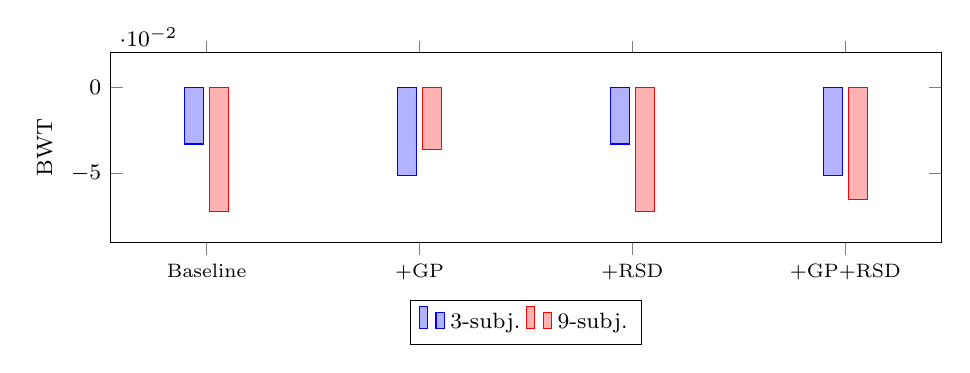
\begin{tikzpicture}
\begin{axis}[
    ybar, bar width=7pt, width=\columnwidth, height=4cm,
    symbolic x coords={Baseline,+GP,+RSD,+GP+RSD}, xtick=data,
    ylabel={BWT}, ymin=-0.09, ymax=0.02,
    legend style={at={(0.5,-0.30)},anchor=north,legend columns=-1,font=\footnotesize},
    enlarge x limits=0.15, tick label style={font=\footnotesize},
    label style={font=\footnotesize}, x tick label style={font=\scriptsize},
]
\addplot coordinates {(Baseline,-0.0329) (+GP,-0.0510) (+RSD,-0.0329) (+GP+RSD,-0.0510)};
\addplot coordinates {(Baseline,-0.0719) (+GP,-0.0360) (+RSD,-0.0719) (+GP+RSD,-0.0648)};
\legend{3-subj., 9-subj.}
\end{axis}
\end{tikzpicture}
\caption{BWT (less negative is better), all configurations, both scales. Baseline/+RSD bars coincide exactly. GP's effect reverses sign between scales.}
\label{fig:bwt}
\end{figure}

\begin{table}[t]
\caption{GP and RSD diagnostics, both scales.}
\label{tab:diag}
\centering
\small
\begin{tabular}{@{}lcccc@{}}
\toprule
& \multicolumn{2}{c}{GP conflict rate} & \multicolumn{2}{c}{RSD final shifts} \\
Config & 3-subj. & 9-subj. & 3-subj. & 9-subj. \\
\midrule
GP / RSD only & 47.2\% & 57.2\% & 10/324 & 243/6210 \\
GP+RSD & --\hphantom{0.0\%} & --\hphantom{0.0\%} & 7/324 & 258/6210 \\
\bottomrule
\end{tabular}
\end{table}

Gradient conflicts are common and more frequent at nine-subject scale (57\% vs.\ 47\% of steps); mean gradient alignment after projection is strongly positive at both scales ($\langle\tilde g,g_M\rangle\approx0.97$--$1.05$, up from negative before projection), confirming GP resolves conflicts as designed at the single-step level -- which does not by itself guarantee the multi-epoch accuracy effect above.

\textbf{Summary answers.} \emph{Does GP help?} Yes, but only at nine-subject scale (BWT $-0.0719\to-0.0360$), at a genuine plasticity/accuracy cost (Avg Acc$(i,i)$ $-4.3$ pts, Avg Acc$(N,i)$ $-1.1$ pts). \emph{Does RSD help?} No, at neither scale, by construction of the current implementation. \emph{Does combining help further?} No: +GP+RSD never beats +GP, and the one place they differ (nine-subject scale) is attributable to RNG noise, not RSD. \emph{Which contributes most?} GP is the only component shown to move any accuracy metric. \emph{Does one hurt another metric?} Yes -- GP's stability gain is not free (above). GP is therefore the component worth further, multi-seed evaluation; RSD needs no further accuracy-level runs until connected to an adaptation mechanism (Section VII).

\subsection{Hyperparameter Sensitivity}
\label{sec:sensitivity}

The codebase's \texttt{run\_sensitivity.py} supports sweeping memory size, learning rate, epochs/subject, batch sizes, or RSD's window/segment-length parameters. Only two sweeps were actually run: memory size (Baseline, +GP) and ER's learning rate, both at three-subject scale, 2--3 points, one seed (Table~\ref{tab:sens}). RSD's own parameters were never swept despite the code supporting it; GP has no continuous hyperparameter beyond the shared memory size (its conflict test is a fixed sign check).

\begin{table}[t]
\caption{Hyperparameter sensitivity (3-subject scale, seed 0).}
\label{tab:sens}
\centering
\small
\begin{tabular}{@{}llccc@{}}
\toprule
Config & Value & BWT & Final Acc \\
\midrule
Baseline & mem=50 & $-$0.0186 & 0.3015 \\
Baseline & mem=200 & $-$0.0329 & 0.3121 \\
+GP & mem=50 & $+$0.0072 & 0.3411 \\
+GP & mem=200 & $-$0.0510 & 0.3016 \\
ER & lr=3e-4 & $+$0.0544 & 0.3094 \\
ER & lr=1e-3 & $-$0.0366 & 0.3112 \\
ER & lr=3e-3 & $+$0.0090 & 0.3822 \\
\bottomrule
\end{tabular}
\end{table}

With 2--3 points, one seed, one scale, this is a directional indicator, not a robustness proof. Notably, +GP's BWT sign flips between memory 50 ($+$0.0072) and 200 ($-$0.0510): the three-subject conclusion ``GP does not help'' (Section VI-A) is itself memory-size-dependent. ER's accuracy rises monotonically with learning rate over the tested range, leaving open whether a larger rate helps further. A real robustness claim needs: more memory-size points across all four configurations, at least one RSD-parameter sweep (entirely absent despite being implemented), the same sweeps at nine-subject scale, and multiple seeds -- none of which were run here due to compute budget (Section VI-F).

\subsection{Sequential Subject Order Analysis}
\label{sec:order}

\textbf{Status: in progress, not yet complete.} \texttt{results/subject\_order/} contained no finished runs in either result snapshot inspected while writing this paper; the reduced-scale experiment described below was launched but had not finished at the time of writing. We report this honestly rather than fabricate order-comparison numbers.

The code already exists and is complete: \texttt{run\_subject\_order.py} trains the same configuration against the canonical order plus \texttt{--num\_orders} random permutations, holding the training seed fixed across orders (a separate \texttt{--order\_seed} controls only the permutations), and aggregates BWT/accuracy mean$\pm$std automatically. Given compute constraints, we recommend a minimal reduced-scale check rather than the full nine-subject sweep: three subjects (A01--A03) rather than four, since three subjects admit only $3!=6$ distinct orderings in total, so canonical order plus five random permutations covers every possible ordering \emph{exhaustively} rather than sampling a small fraction of a much larger permutation space, at no extra cost over a partial sweep. We run this for Baseline and +GP (the only configuration shown to change accuracy metrics), at the same three-epoch budget as the rest of the three-subject-scale ablation, giving 12 runs (2 configurations $\times$ 6 orders) directly comparable to the canonical-order numbers already reported in Table~\ref{tab:ablation}. This experiment was in progress at the time of writing; until it completes, whether this study's ablation conclusions are an artifact of the canonical A01$\to$A09 order remains a genuine open question, and we report no order-comparison numbers here.

\subsection{Comparison with ER and MIR}
\label{sec:ermir}

\begin{table}[t]
\caption{Full comparison, three-subject scale, seed 0.}
\label{tab:comparison}
\centering
\small
\begin{tabular}{@{}lccc@{}}
\toprule
Method & BWT & Final Acc \\
\midrule
Baseline & $-$0.0329 & 0.3121 \\
+GP & $-$0.0510 & 0.3016 \\
+RSD & $-$0.0329$^{*}$ & 0.3121$^{*}$ \\
+GP+RSD & $-$0.0510$^{*}$ & 0.3016$^{*}$ \\
ER & $-$0.0366 & 0.3112 \\
MIR & $-$0.0622 & 0.2840 \\
GMED & $-$0.0503 & 0.3074 \\
\bottomrule
\end{tabular}
\end{table}

At three-subject scale, plain Baseline MUDVI has the best BWT and near-best accuracy of every method compared, including GP, RSD, ER, MIR, and GMED; none improves on it. At nine-subject scale, only ER is fully comparable: BWT $-0.0419$, Avg Acc$(N,i)$ 0.3108. MIR's nine-subject run is incomplete (5/9 subjects checkpointed, no final metrics, resumable but not finished within budget); GMED was never run at nine-subject scale. Where comparable: by BWT, +GP ($-0.0360$) beats ER ($-0.0419$), reversing the three-subject ranking; by accuracy, ER (0.3108) beats every MUDVI-family configuration (Baseline/+RSD 0.2938, +GP 0.2825, +GP+RSD 0.2595) -- GP is not an unqualified improvement over this cheap baseline, only a stability one.

\subsection{Computational Cost}
\label{sec:cost}

All nine-subject/15-epoch runs execute 6210 steps (three-subject/3-epoch: 324), identical across the four MUDVI-family configurations. GP's two-backward-pass design would, in principle, roughly double per-step backward cost; the \emph{measured} overhead is far smaller (+4.4\% wall-clock at nine-subject scale vs.\ Baseline's 3582\,s), indicating backward-pass compute is not this setup's bottleneck. RSD's single-run timing is not a reliable cost estimate (+RSD measured 7.0\% \emph{faster} than Baseline, +GP+RSD 9.4\% slower than Baseline, i.e.\ only $\sim$5 points more than +GP) -- with one run per configuration on a shared Lightning AI instance we cannot separate RSD's true cost from ordinary timing noise. The five completed nine-subject runs (Baseline, +GP, +RSD, +GP+RSD, ER) consumed $\approx$4.60 GPU-hours total; this budget is the direct reason the subject-order analysis and a fuller sensitivity sweep were not run at nine-subject scale, and why MIR's nine-subject run was left incomplete. Practically: GP's roughly-halved BWT costs about 4\% more compute and a measurable accuracy drop -- favorable if stability is the priority; RSD's cost is unresolved but moot, since it currently buys no measured benefit at all (Section VI-A).

\section{Limitations and Future Work}

\textbf{Single seed, RNG-isolation confound.} All results use one run per configuration; we report point estimates, not statistics. GP's code path skips a batch-reshuffle step the baseline performs, so baseline-vs-GP differences (and the +GP+RSD vs.\ +GP gap, Section VI-A) are not perfectly isolated from random batch order -- disclosed rather than silently accepted; fixing it (independent, identically-seeded shuffling per code path) is a direct next step.

\textbf{Scale and coverage gaps.} The three-subject stage is not representative of nine-subject behavior (Section VI-A shows they disagree in direction for GP); hyperparameter sensitivity covers only 2--3 points per sweep at one scale (Section VI-C); subject-order robustness is entirely untested despite being fully supported by the codebase (Section VI-D) -- the reduced-scale experiment specified there is the recommended next step before any order-robustness claim.

\textbf{RSD is diagnostic only.} It does not currently influence training or the memory buffer. Connecting it to an adaptation mechanism (e.g., gating the memory-update rule on a detected shift) is the most direct way to test whether shift detection itself, beyond logging, can help.

\textbf{Dataset generalization.} All results are specific to BCI IV 2a training-session files; we make no claim about other EEG datasets or the unusable evaluation-session data.

\section{Conclusion}

Under a controlled four-configuration ablation at both three- and nine-subject scale, gradient projection reduced backward transfer at nine-subject scale (BWT $-0.0719\to-0.0360$) at a real plasticity/accuracy cost, did not help at three-subject scale, and out-stabilized (but did not out-accuracy) a same-protocol ER baseline at nine-subject scale. Relationship-shift detection passed its own statistical checks but, verified by code inspection and exact numerical equality at both scales, has no effect on any accuracy metric because it is not connected to any adaptation mechanism -- reported honestly as a diagnostic contribution, not a learning improvement. A limited sensitivity check showed GP's benefit is itself memory-size-dependent, and a subject-order robustness analysis -- fully supported by the existing codebase -- was not run within this study's compute budget; we specify the smallest scientifically meaningful version of that experiment rather than assume the result. Future work should prioritize that subject-order check, the RNG-isolation fix, multi-seed GP evaluation, and connecting RSD's signal to an actual adaptation mechanism.

\bibliographystyle{IEEEtran}
\bibliography{references}

\end{document}
